% ------------------------------------------------------------------
%  AETIA -- multimodal pathogen selection from mNGS and clinical evidence
%  Manuscript draft.  Build:  latexmk -pdf main.tex   (or `make` in this folder)
% ------------------------------------------------------------------
\documentclass[11pt,a4paper]{article}

\usepackage[utf8]{inputenc}
\usepackage[T1]{fontenc}
\usepackage{lmodern}
\usepackage[margin=2.5cm]{geometry}
\usepackage{setspace}
\usepackage{graphicx}
\usepackage{amsmath}
\usepackage{booktabs}
\usepackage{xspace}
\usepackage{xcolor}
\usepackage{lineno}
\usepackage[super,sort&compress,numbers]{natbib}
\usepackage[hidelinks]{hyperref}
\usepackage{url}

\graphicspath{{figures/}}
\bibliographystyle{naturemag}
\setcitestyle{super,open={},close={}}

% ---------- names / editorial macros ----------
\newcommand{\toolname}{AETIA\xspace}              % external research-system name (docs/OBER_NAMING.md)
\newcommand{\toolexpansion}{Agentic Evidence Tracing of Infectious Aetiology\xspace}  % expanded at first use in the abstract and Introduction
\newcommand{\mngs}{mNGS\xspace}
\newcommand{\filmarray}{FilmArray\xspace}
\newcommand{\rfive}{R5\xspace}
\newcommand{\vtwenty}{v20\xspace}
\newcommand{\gptsol}{GPT-5.6 Sol\xspace}
\newcommand{\gptluna}{GPT-5.6 Luna\xspace}
\newcommand{\gptterra}{GPT-5.6 Terra\xspace}
\newcommand{\gptastra}{GPT-6 Astra\xspace}
\newcommand{\kmuh}{KMUH\xspace}
\newcommand{\tvgh}{TVGH\xspace}
\newcommand{\tsgh}{TSGH\xspace}
\newcommand{\todo}[1]{\textcolor{red}{[#1]}}     % items to verify before submission

% Title (Nature style: declarative, no colon, states the advance and its consequence).
% Alternatives:
%  (a) Rule-governed, literature-grounded integration of metagenomic and clinical evidence identifies causative pathogens with auditable reasoning
%  (b) Structured multimodal reasoning turns metagenomic pathogen lists into actionable, traceable diagnoses
%  (c) Clinically contextualized multi-agent reasoning outperforms direct large-language-model diagnosis on metagenomic data
\title{Auditable multimodal integration of metagenomic sequencing and clinical evidence identifies causative pathogens in lower respiratory tract infection}

\author{%
\todo{Yu-Cheng Wu}$^{1}$, \todo{Chun-Ting Chang}$^{1}$, \todo{Yuan-Ting Chung}$^{1}$,\\
\todo{Yuan-Ting Yeh}$^{1}$, \todo{clinical co-authors, KMUH}$^{2}$, \todo{clinical co-authors, TVGH}$^{3}$,\\
\todo{clinical co-authors, TSGH}$^{4}$,\\
Yao-Ting Huang$^{1,\ast}$\\[4pt]
\small $^{1}$Department of Computer Science and Information Engineering, National Chung Cheng University, Chiayi, Taiwan\\
\small $^{2}$\todo{Kaohsiung Medical University Hospital, Kaohsiung, Taiwan}\\
\small $^{3}$\todo{Taipei Veterans General Hospital, Taipei, Taiwan}\\
\small $^{4}$\todo{Tri-Service General Hospital, Taipei, Taiwan}\\
\small $^{\ast}$Correspondence: ythuang@cs.ccu.edu.tw}
\date{}

\begin{document}
\sloppy
\onehalfspacing
\linenumbers
\maketitle

\begin{abstract}
Metagenomic next-generation sequencing (\mngs) detects nearly every organism in a respiratory specimen, but most of what it reports is colonizing, contaminating or reactivated rather than causative, and the physician is left to reconcile a long organism list with cultures, multiplex PCR, antigen tests, imaging, blood counts and host status. Here we present \toolname (\toolexpansion), a pipeline that turns this multimodal record into a short, traceable list of causative pathogens. Modality-specific language-model agents extract structured evidence from each test; a deterministic scorer grades every \mngs organism by read burden, within-specimen dominance, control-subtracted rank, specimen alignment and same-organism hospital support, and applies pre-specified guardrails against known colonizers; a language-model safety review flags what the rules did not pick; and a final rule rescues a candidate only when PubMed literature judged against the patient's own site, syndrome and host, or definitive direct evidence, supports it. Selection is frozen before any rationale is written, and every decision carries its rule path and source hashes. On \todo{55} patients with suspected lower respiratory tract infection from three Taiwanese hospitals, \toolname reached a precision of \todo{71.6\%}, recall of \todo{91.4\%} and F1 of \todo{80.3\%} against physician-adjudicated pathogens, compared with F1 of \todo{14.8\%} for the raw \mngs report, \todo{50.0\%} for \filmarray and galactomannan testing and \todo{45.5\%} for culture, and, in an earlier 35-patient intensive-care series, reducing the average number of organisms presented per patient from \todo{5.8} to \todo{2.0}. On \todo{41} patients, the same pipeline exceeded four frontier language models prompted directly with the identical raw data by \todo{14--15} F1 points, mainly through recall (\todo{90.8\%} versus \todo{57--61\%}). \toolname is research software whose output is a reviewed candidate list, not a diagnosis; it shows that structured, literature-grounded integration, rather than end-to-end prompting, is what makes \mngs clinically interpretable.
\end{abstract}

\section*{Introduction}
% ------------------------------------------------------------------
% Introduction (no subsections; published literature only)
% ------------------------------------------------------------------

Lower respiratory tract infection is frequently treated without a microbiological diagnosis. In a large prospective study of adults admitted with community-acquired pneumonia, no pathogen was identified in 62\% despite extensive conventional testing\cite{jain2015community}. In critically ill patients, previous antibiotic treatment further reduces culture sensitivity\cite{miao2018microbiological}, noninfectious inflammatory syndromes can resemble pneumonia\cite{langelier2018integrating}, and the differential diagnosis extends to fungi, viruses and opportunistic pathogens. Metagenomic next-generation sequencing (\mngs) was developed to address this gap by detecting bacterial, fungal, viral and parasitic nucleic acids without a prespecified target\cite{chiu2019clinical,simner2018understanding}. Clinical studies have shown its diagnostic potential in meningoencephalitis\cite{wilson2019clinical}, bloodstream infection\cite{blauwkamp2019analytical,hogan2021clinical} and lower respiratory tract infection\cite{charalampous2019nanopore,langelier2018integrating,chen2020clinical,diao2022metagenomics}, and the assay is increasingly used in critically ill patients in Asia\cite{miao2018microbiological,han2019mngs}. Its breadth, however, carries a clinical risk: tests that detect incidentally carried microbes can lead to antimicrobial overuse and adverse outcomes\cite{mick2023integrated}.

The main challenge is interpretation rather than detection. Respiratory \mngs identifies upper-airway flora\cite{charlson2011topographical,dickson2016microbiome}, reagent and environmental contaminants\cite{salter2014reagent}, herpesviruses shed or reactivated during critical illness\cite{luyt2007herpes,limaye2008cytomegalovirus} and airway-colonizing \textit{Candida}\cite{meersseman2009significance}, as well as causative pathogens. In a prospective bronchoalveolar-lavage cohort, \mngs identified a definite or probable pathogen in 65\% of patients with lower respiratory tract infection, compared with 20\% by culture, but had a specificity of 75.4\% and a positive predictive value of 78.5\% against a composite reference standard\cite{chen2020clinical}. Distinguishing infection from colonization therefore remains a central limitation\cite{simner2018understanding,diao2022metagenomics}. Read thresholds and subtraction of no-template controls reduce background signal but do not resolve the biological ambiguity of a colonized respiratory specimen\cite{miller2019laboratory,schlaberg2017validation}.

Resolving that ambiguity requires evidence from outside the sequencing assay. Culture establishes viability and enables susceptibility testing\cite{metlay2019diagnosis,kalil2016management}, multiplex PCR provides rapid, validated target-specific results\cite{buchan2020practical}, galactomannan contributes an independent criterion for invasive fungal disease\cite{donnelly2020revision}, serology can establish infection after the organism has cleared from the airway\todo{cite}, and imaging defines the anatomical syndrome of pneumonia\cite{metlay2019diagnosis}. Each result must be read against the specimen and its timing: infection confined to blood, tissue, an abscess or an empyema may be absent from respiratory fluid, and intermittent or treated infection may be missed outside its detection window\cite{gu2019clinical,miller2022role,schlaberg2017validation}. Determining causation consequently requires integration of sequencing, conventional microbiology and clinical context.

Computational approaches to this problem have so far drawn only on the sequencing data. A rules-based model that scored organisms by relative abundance and known pathogenicity separated pathogens from commensals in tracheal aspirates from critically ill adults\cite{langelier2018integrating}, and classifiers adding host gene expression improved diagnosis of lower respiratory tract infection in critically ill children\cite{mick2023integrated} and of sepsis from plasma\cite{kalantar2022integrated}. Their host-response components require RNA sequencing of host transcripts, and none incorporates culture, antigen or serological results or the clinical course that physicians use to adjudicate causation.

Large language models could perform this integration because they encode clinical knowledge\cite{singhal2023large}, generate differential diagnoses from vignettes\cite{mcduff2025towards,tu2025towards} and have been evaluated as infectious-diseases consultants\cite{maillard2024chatbot}. Their performance on curated tasks, however, has not consistently transferred to clinical records. In an evaluation of 2,400 patient cases, current models performed worse than physicians, did not reliably follow diagnostic or treatment guidelines, had difficulty interpreting laboratory results and were sensitive to both the quantity and the order of the information they received\cite{hager2024evaluation}. Model outputs also vary between runs and may not reveal which evidence determined a prediction\cite{ji2023survey}. A generated explanation cannot by itself establish fidelity because a model's stated reasoning may not correspond to the computation that produced its answer\cite{turpin2023language}; in clinical applications, such post-hoc explanations can provide false reassurance\cite{ghassemi2021false}. Multi-agent systems\cite{tang2024medagents,kim2024mdagents,qiu2024llm} and retrieval augmentation\cite{lewis2020retrieval,xiong2024benchmarking} address parts of this problem, but clinical use also requires reproducible decisions, traceable evidence and an explanation written separately from the prediction. Evaluation must also guard against leakage\cite{kapoor2023leakage}: clinical notes often record the treating team's final diagnosis, which a model can copy rather than infer. To our knowledge, no approach has combined \mngs with conventional microbiology and the clinical record to attribute causation organism by organism under these constraints.

Here we present \toolname (\toolexpansion), which integrates respiratory \mngs with conventional microbiology and clinical data. Modality-specific language-model agents extract structured evidence; deterministic rules select candidate pathogens; and case-matched PubMed evidence can rescue candidates not selected initially. The clinical rationale is written only after the selected list has been fixed. In patients with suspected lower respiratory tract infection from three medical centres in Taiwan, we compared \toolname with individual diagnostic read-outs and with direct prompting of general-purpose language models against physician-adjudicated pathogens. \toolname identified the adjudicated pathogens more accurately than any single read-out or directly prompted model, reported far fewer organisms than the sequencing report while retaining most true pathogens, and linked each selection and exclusion to the evidence behind it. The system is intended to provide an evidence-linked candidate list for physician review, not an autonomous diagnosis.


\begin{figure}[p]
  \centering
  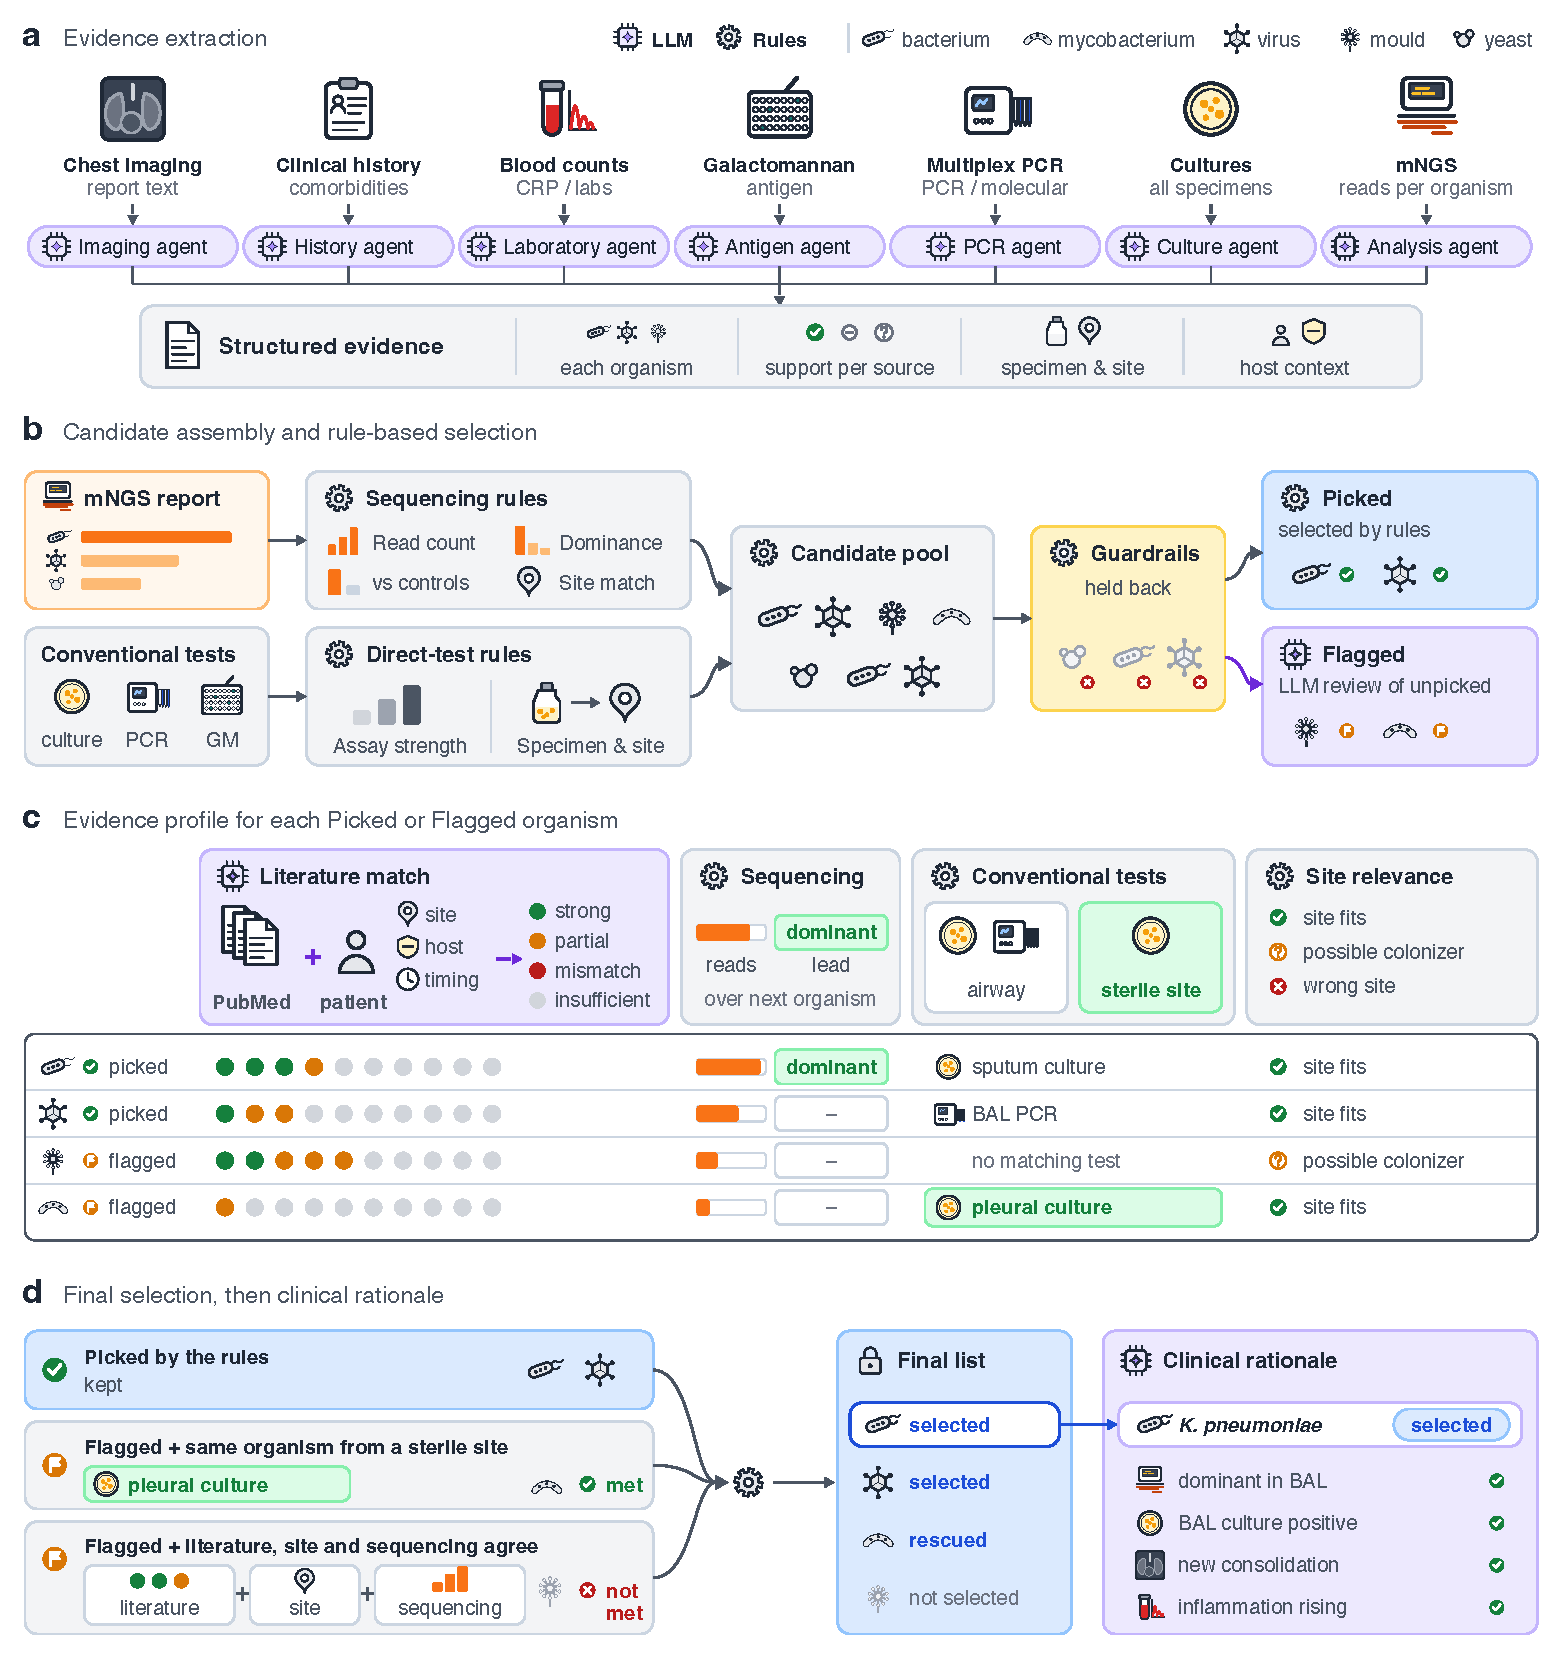
\includegraphics[width=\textwidth]{fig1_overview}
  \caption{\textbf{Overview of \toolname.}
  \textbf{a}, One patient's record. Seven read-outs are each parsed by a dedicated language-model agent into a fixed schema; glyphs mark the organism classes (bacterium, fungus, virus, yeast) or host context an agent supplies. Agents see neither the reference labels nor each other.
  \textbf{b}, Deterministic selection. Organisms on the \mngs report (bars, reads; R0--R4, read tier) pass four filters---read burden, within-specimen dominance, control-subtracted rank, and site alignment with same-organism hospital support---that assign a signal tier and a causative level; 33 guardrails demote colonizers and reactivation viruses (crossed glyphs). Levels 1--2 and supported level 3 are picked in a fixed order. A language-model review reads only the unpicked organisms and can flag them (high priority, context needed) but cannot pick.
  \textbf{c}, Evidence for each carried candidate: A, PubMed articles judged for exact-species, site-matched human evidence and re-judged against the patient (A1 case-fit); B, \mngs strength on an absolute and a relative axis; C, direct non-\mngs evidence graded C0--C3; D, colonization gate (reported, not gating).
  \textbf{d}, Rule \rfive selects organisms that were picked, meet C3, or meet A1, site alignment and a B axis together. The list is frozen with rule paths and input hashes before a language model writes the rationale; delivery is a summary table with a traceable JSON, Markdown and XLSX package.}
  \label{fig:overview}
\end{figure}

\section*{Results}
% ------------------------------------------------------------------
%  Results.  Declarative subsection headings; each states a finding.
%  Every number that comes from the student slides rather than from the
%  evaluation JSON is wrapped in \todo{} (see README, "Before submission").
% ------------------------------------------------------------------

\subsection*{\toolname separates evidence extraction, rule-based selection and literature-grounded rescue}

\toolname takes, for one patient, the standardized record of nine sources: admission diagnosis, underlying conditions, blood counts, other laboratory values, cultures, \filmarray results, galactomannan, imaging reports and the laboratory's \mngs report with per-organism read counts and no-template-control codes (Fig.~\ref{fig:overview}a). Each modality is read by its own language-model agent into a fixed JSON schema. The agents are single-purpose: the imaging agent sees only imaging, the culture agent only cultures, and none of them sees the answer labels. A deterministic summary then joins the per-modality outputs into organism-level support and a host-vulnerability tier.

Selection is deterministic (Fig.~\ref{fig:overview}b). Every organism on the \mngs report is ranked by its control-subtracted priority and read percentile, tiered by read burden (R0--R4, decade thresholds from 1 to 10,000 reads) and by dominance within the specimen (D3 when the top organism has at least ten times the reads of the runner-up), aligned with the target site, and joined with same-organism hospital evidence. These features map to an \mngs signal tier (M1 strong to M5 background) and, together with site alignment and host status, to one of five causative levels. Pre-specified guardrails demote respiratory \textit{Candida}, oral and upper-airway flora, water-borne Gram-negative environmental organisms, skin flora, Epstein--Barr virus and other low-actionability herpesviruses, weak mould signals and generic hospital labels. Level~1--2 organisms and level~3 organisms with a protected or supported rationale are picked, in a fixed order that no later stage may change. A language-model safety review then examines only the unpicked organisms and sorts them into high-priority, context-needed, low-specificity or omitted; the first two tiers, and only those, are carried forward.

For every carried candidate, four evidence modules are computed (Fig.~\ref{fig:overview}c). Module A retrieves up to ten PubMed articles for the organism at the target site and judges each for exact-species, human, site-matched causal evidence with a quoted supporting span; module A1 re-judges every article against the patient---site, syndrome, host, phenotype and timing---and returns strong match, partial match, mismatch or insufficient. Module B scores \mngs strength on an absolute axis (signal tier M1--M2 or read tier R3--R4) and a relative axis (dominance D2--D3, or rank~1 with read percentile $\ge 0.8$). Module C grades same-organism non-\mngs evidence from C0 (none) to C3 (exact organism in a sterile-site or tissue specimen), and module D applies a specimen-colonization gate. Missing or pending tests are treated as unknown, never as negative. The final rule \rfive (Fig.~\ref{fig:overview}d) keeps every upstream pick and rescues a candidate only if C3 holds, or if A1 (at least two strong matches, or at least seven strong plus partial) coincides with site alignment and at least one B axis. Only then is a rationale written, by a language model constrained to the frozen selection and the patient's evidence window, and audited for structure before delivery as a simple table and a traceable JSON, Markdown and XLSX package.

\subsection*{\toolname identifies causative pathogens more accurately than any single conventional read-out}

We evaluated \toolname on \todo{55} patients with suspected lower respiratory tract infection from Kaohsiung Medical University Hospital (\kmuh, $n=\todo{30}$), Taipei Veterans General Hospital (\tvgh) and Tri-Service General Hospital (\tsgh; together $n=\todo{25}$), drawn from a three-hospital \mngs registry of 105 specimens (Table~\ref{tab:cohort}; Supplementary Fig.~1). Patients were predominantly critically ill (71\% in intensive care at sampling), 56\% had hospital- or ventilator-associated pneumonia, 37\% had an active malignancy and 39\% were receiving systemic corticosteroids; 60\% of \mngs specimens were bronchoalveolar lavage fluid. The reference standard was the causative pathogen list adjudicated by the treating infectious-diseases physicians, with versioned label revisions (Methods). Because a patient may have more than one pathogen, we scored (patient, organism) pairs at exact species level with a frozen synonym table and report micro-averaged precision, recall and F1.

\toolname reached a precision of \todo{71.6\%}, a recall of \todo{91.4\%} and an F1 of \todo{80.3\%} (Fig.~\ref{fig:benchmark}a,b). The raw \mngs report, scored by taking every listed organism as a call, had the highest recall (\todo{93.1\%}) but a precision of \todo{8.0\%} (F1 \todo{14.8\%}): the report contains the pathogen almost every time, but for every causative organism it names it lists about \todo{eleven} that are not \todo{(1--0.08)/0.08; confirm FP count from the evaluation JSON}. The targeted tests behaved in the opposite way. \filmarray and galactomannan together had a precision of \todo{67.6\%} but a recall of \todo{39.7\%} (F1 \todo{50.0\%}), and culture reached \todo{48.1\%} precision and \todo{43.1\%} recall (F1 \todo{45.5\%}). \toolname therefore kept essentially all of the sensitivity of \mngs while raising its precision by \todo{ninefold}, and it exceeded the precision of the targeted tests without their blind spots for fungi, viruses and fastidious organisms. \todo{Add per-hospital metrics, exact-set-match rate and any-hit rate from the evaluation JSON; add 95\% confidence intervals by patient-level bootstrap.}

\subsection*{\toolname reduces the organism burden presented to the physician}

The clinical cost of \mngs is not only false attribution but the length of the list a physician must reconcile. In an earlier series of \todo{35} intensive-care patients from \kmuh evaluated with the first version of the pipeline, culture reported at least one organism in \todo{24\%} of patients and \filmarray in \todo{64\%}, whereas \mngs reported at least one organism in every patient, with a mean of \todo{5.76} organisms per patient (Fig.~\ref{fig:benchmark}c,d). \toolname retained a call in every patient but presented a mean of \todo{1.97} organisms, close to the \todo{one to two} pathogens per patient in the adjudicated reference. The reduction is not a fixed cut-off: it comes from the demotion of colonizers, contaminants and reactivation viruses that fail the site, dominance and support rules, and from the guardrails that hold respiratory \textit{Candida} and oral flora below the picking threshold unless independent evidence exists. \todo{Confirm the relation of this 35-patient series to the 55-patient cohort and recompute organisms per patient for the 55 from the R5 decisions (518 candidates $\rightarrow$ 123 selected, i.e. 9.4 $\rightarrow$ 2.2 per patient).}

\subsection*{Structured integration outperforms direct prompting of frontier language models}

To test whether the gain comes from the structure of the pipeline rather than from the language models inside it, we gave four frontier models (\gptsol, \gptluna, \gptterra and \gptastra) exactly the raw data that \toolname receives---the \mngs list with reads and control codes, cultures, \filmarray, galactomannan, molecular tests, imaging reports, blood counts, diagnosis and underlying conditions---for \todo{41} patients (\kmuh $n=\todo{30}$, \tvgh/\tsgh $n=\todo{11}$), de-identified, with a single expert-written prompt that explained the colonization and site rules in words, a JSON output schema and medium reasoning effort, and no retrieval, candidate pool or answer key (Methods; Supplementary Note~\todo{2}). Predictions were frozen before the reference labels were read.

All four models converged on the same operating point: precision between \todo{67.7\%} and \todo{70.5\%}, recall between \todo{56.6\%} and \todo{60.5\%}, and F1 between \todo{62.4\%} and \todo{63.9\%} (Fig.~\ref{fig:llm}). On the same \todo{41} patients, \toolname reached a recall of \todo{90.8\%} at a precision of \todo{67.7\%} (\todo{69} true positives, \todo{33} false positives, \todo{7} false negatives), for an F1 of \todo{77.5\%}, \todo{13.6--15.1} points above the best direct-prompting model. The difference is almost entirely recall: prompted with the same warnings about colonization that \toolname encodes as rules, the models declined to call organisms that the rules, the hospital evidence and the case-matched literature together supported, whereas their precision was no better than the pipeline's. \todo{Slide 3 lists the pipeline's precision on these 41 patients as 71.62\%; the frozen tally TP 69 / FP 33 gives 67.65\%, and the slide's recall and F1 match that tally. Resolve from reports/idfixed\_20260906 before submission.} The newest model (\gptastra) improved recall by only \todo{2.6} points over its predecessors, which suggests that the shortfall is not a matter of model capacity but of what a single prompt can be made to do with a long, noisy organism list.

\subsection*{Rescue by case-matched literature contributes a minority of selections}

Across the \todo{55} patients, the deterministic scorer considered \todo{518} organism candidates and picked \todo{114}; the \rfive rule rescued a further \todo{9}, giving \todo{123} selected organisms (\todo{2.2} per patient). Rescue therefore changed \todo{7\%} of the final list, and every rescued organism carries its rule path (C3 direct, or A1 threshold with site alignment and B axis) and the PubMed identifiers of the articles that met the case-fit thresholds. \todo{From the evaluation JSON: how many of the 9 rescued organisms were true positives; how many false negatives remained and why (not in report, below read tier, guardrail); how many false positives were upstream picks versus rescues.} The immutability of upstream picks means that rescue can only add recall; the precision of the final list is bounded by the deterministic stage.

\subsection*{Decisions are traceable to their evidence}

Two cases illustrate the output (Supplementary Note~\todo{3}; details anonymized). In a patient with new bilateral consolidation and pleural effusions, a rising C-reactive protein and worsening hypoxaemia, the \mngs report listed \textit{Klebsiella pneumoniae} with \todo{68,569} reads alongside \textit{Candida albicans}; \toolname selected \textit{K.~pneumoniae} (dominant, aligned, supported by imaging and inflammatory markers) and excluded \textit{C.~albicans} as respiratory colonization with low read counts and repeated low-burden culture. In a second patient, \textit{Candida tropicalis} was selected despite the general demotion of respiratory yeasts, because multiple blood-culture sets were positive for the same species and the bronchoalveolar \mngs reads were high, which satisfies the C3 direct-evidence path. \todo{Both vignettes come from the January 2026 prototype (talk slide 15); regenerate them from the AETIA R5 rationale outputs for the same patients.} In each case the delivered record names the rule that fired, the modules that supported or opposed each organism, and the SHA-256 hash of every input file, so that a reviewer can reproduce the decision and see exactly which finding decided it.

\subsection*{The pipeline is reproducible offline}

All \todo{55} frozen \rfive decisions were replayed from the frozen upstream, case-fit and clinical inputs and were byte-identical to the delivered files. The 41-patient direct-prompting comparison was likewise rescored from \todo{164} frozen model outputs with identical metrics. The public code passes \todo{319} Python and \todo{8} Node offline tests that cover format processing, the deterministic scorer, the review, literature, case-fit and clinical rules, \rfive, rationale handoff, delivery and multi-cohort patient-identity isolation; the test harness blocks network access and strips API keys, so no test depends on a paid model or on live PubMed. The current scorer (\vtwenty) reproduces the picked set of every one of the \todo{55} patients scored with the version used for the reported results (v19), while changing candidate levels in \todo{15} and pick order in \todo{5} patients (Supplementary Note~\todo{4}).


\begin{figure}[p]
  \centering
  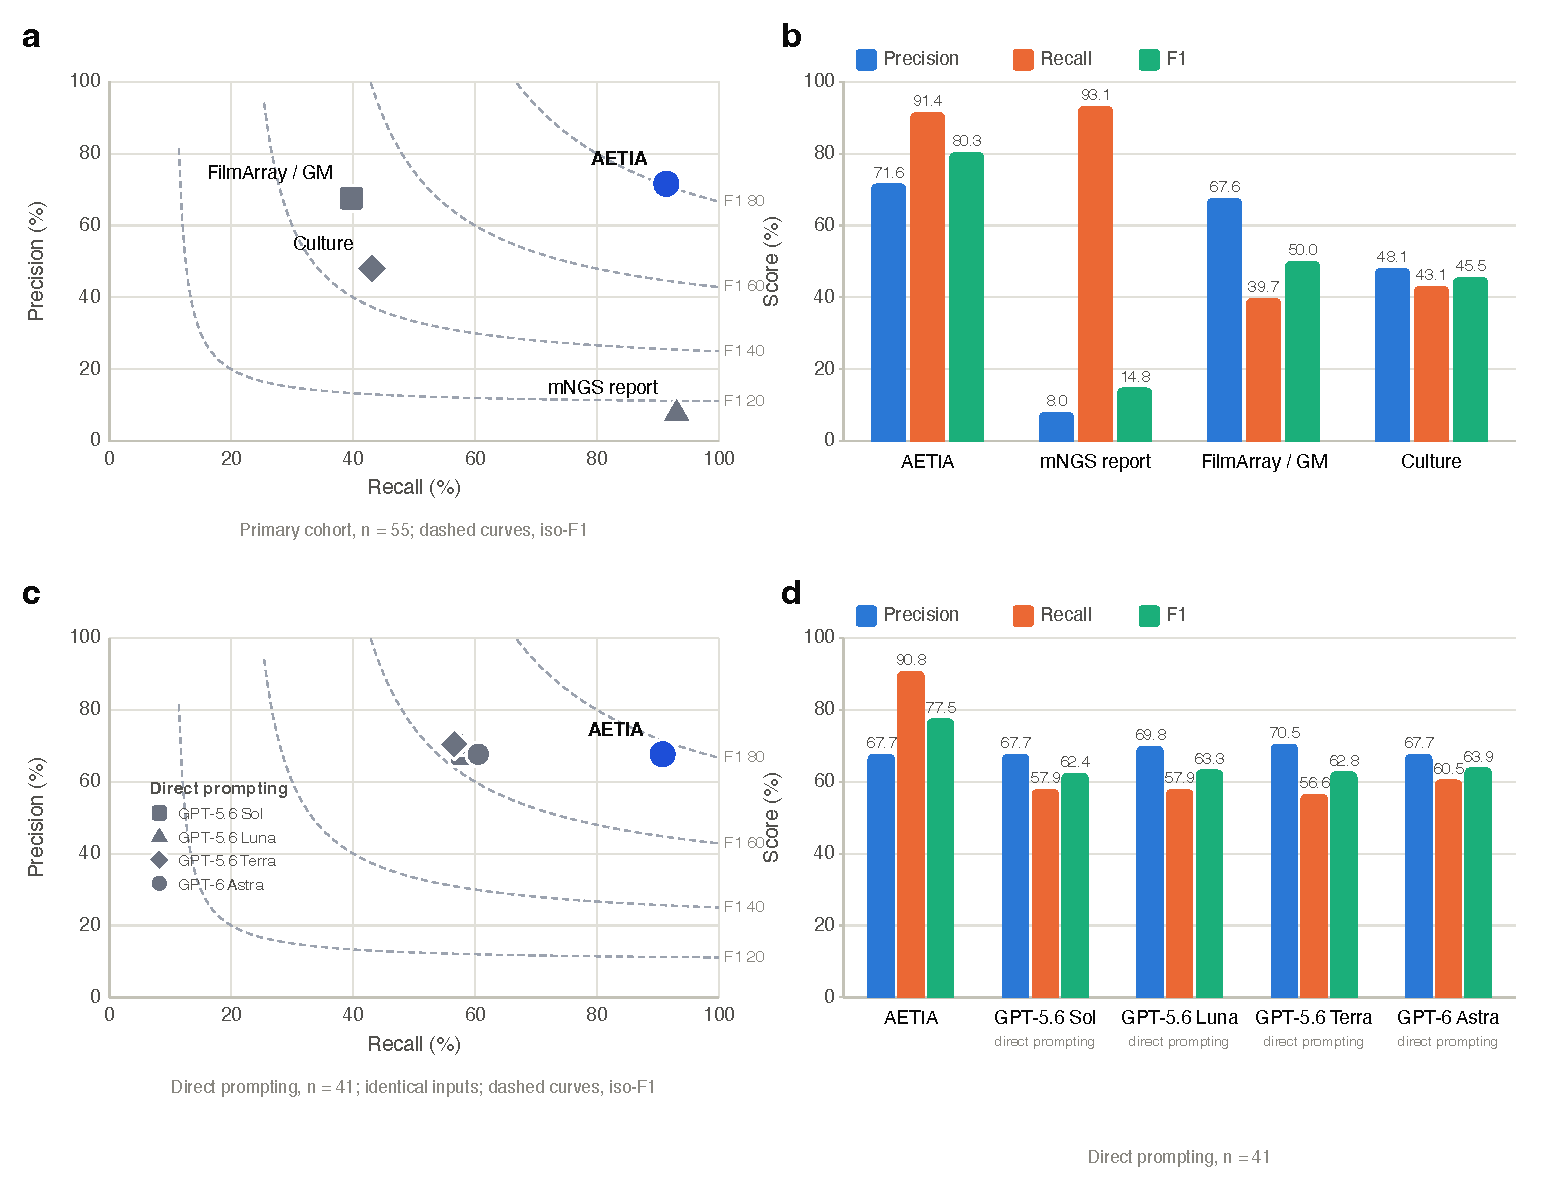
\includegraphics[width=0.9\textwidth]{fig2_benchmark}
  \caption{\textbf{Pathogen selection compared with the raw \mngs report, \filmarray/galactomannan and culture.}
  \textbf{a}, Precision against recall for \toolname (blue) and for each read-out taken at face value: all organisms in the \mngs report (triangle), all positive \filmarray or galactomannan targets (square) and all cultured organisms (diamond); dashed curves, constant F1.
  \textbf{b}, The same comparison as precision, recall and F1. $n=\todo{55}$ patients (\kmuh \todo{30}; \tvgh and \tsgh \todo{25}); unit, (patient, organism) pair at species level; reference standard, physician-adjudicated pathogens (Methods).
  \textbf{c},\textbf{d}, Earlier intensive-care series (\kmuh, $n=\todo{35}$; first pipeline version): fraction of patients with at least one reported organism (\textbf{c}) and mean organisms per patient (\textbf{d}). \todo{Values transcribed from slides; regenerate from the evaluation output.}}
  \label{fig:benchmark}
\end{figure}

\begin{figure}[p]
  \centering
  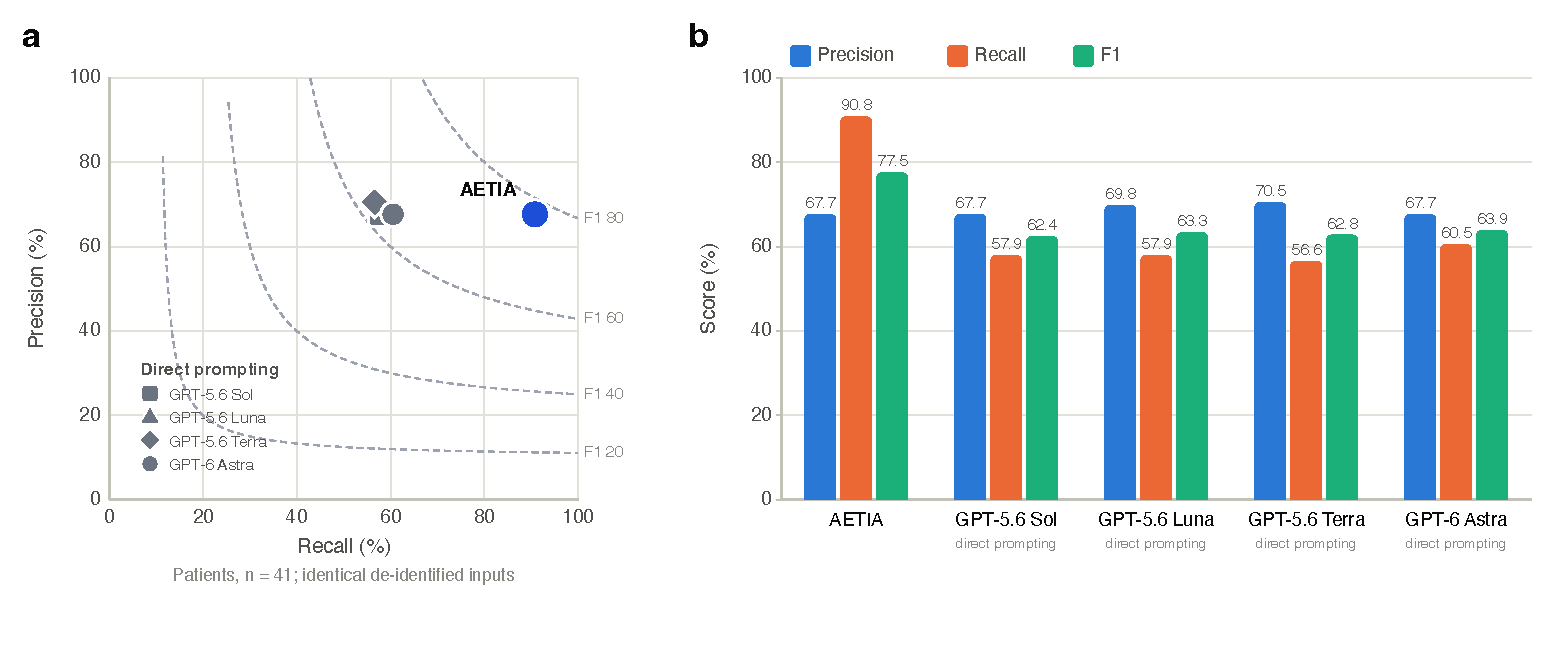
\includegraphics[width=0.9\textwidth]{fig3_llm_comparison}
  \caption{\textbf{Comparison with frontier language models prompted directly on the same data.}
  \gptsol, \gptluna, \gptterra and \gptastra received the identical de-identified record---raw \mngs list with reads and control codes, cultures, \filmarray, galactomannan, molecular tests, imaging reports, blood counts and diagnoses---with one prompt, a JSON schema and no retrieval or reference labels (Methods; Supplementary Note~\todo{2}).
  \textbf{a}, Precision against recall; \toolname in blue, models in grey (marker key in panel); dashed curves, constant F1.
  \textbf{b}, Precision, recall and F1. $n=\todo{41}$ patients (\kmuh \todo{30}; \tvgh and \tsgh \todo{11}); micro-averaged over (patient, organism) pairs; \toolname values from the frozen \rfive decisions on the same patients (TP~\todo{69}, FP~\todo{33}, FN~\todo{7}). \todo{Slide gives 71.62\% precision; TP/FP imply 67.65\%.}}
  \label{fig:llm}
\end{figure}

% Generated by tables/make_table1.py from the cohort workbook (kept outside the repo). Do not edit by hand.
\begin{table}[p]
\centering
\caption{\textbf{Characteristics of the three-hospital \mngs registry.} The 105-specimen registry from which the 55- and 41-patient evaluation cohorts were drawn (Extended Data Fig.~\ref{fig:ed1}). Values are $n$ (\%) or median (interquartile range).}
\label{tab:cohort}
\small
\begin{tabular}{lr}
\toprule
Characteristic & All patients ($n=105$) \\
\midrule
\textit{Hospital} & \\
\quad KMUH & 51 (48.6\%) \\
\quad TVGH & 35 (33.3\%) \\
\quad TSGH & 19 (18.1\%) \\
Age, years & 69 (56--75) \\
Male sex & 68 (64.8\%) \\
Current or former smoker & 19 (18.1\%) \\
Intensive care unit at sampling & 75 (71.4\%) \\
\textit{Underlying conditions} & \\
\quad Diabetes mellitus & 29 (27.6\%) \\
\quad Chronic kidney disease & 16 (15.2\%) \\
\quad End-stage renal disease on dialysis & 4 (3.8\%) \\
\quad Liver cirrhosis & 1 (1.0\%) \\
\quad Autoimmune disease & 6 (5.7\%) \\
\quad Active malignancy & 39 (37.1\%) \\
\quad Systemic corticosteroids$^{\dagger}$ & 40 (38.5\%) \\
\quad ARDS on the day of sampling$^{\dagger}$ & 48 (46.6\%) \\
\textit{Pneumonia category} & \\
\quad Community-acquired & 21 (20.0\%) \\
\quad Hospital- or ventilator-associated & 59 (56.2\%) \\
\quad Not classified & 25 (23.8\%) \\
PaO$_2$/FiO$_2$ ratio at sampling & 200 (152--302) \\
\textit{\mngs specimen} & \\
\quad BALF & 63 (60.0\%) \\
\quad Blood & 24 (22.9\%) \\
\quad Sputum & 4 (3.8\%) \\
\quad CSF & 6 (5.7\%) \\
\quad Tissue & 5 (4.8\%) \\
\quad Other & 3 (2.9\%) \\
Organisms per \mngs report, median (IQR) & 4 (1--6) \\
\mngs report with no organism & 8 (7.6\%) \\
Any positive culture & 69 (65.7\%) \\
\textit{Clinical course} & \\
\quad Antimicrobial therapy changed & 69 (65.7\%) \\
\quad \quad Escalation & 49 (46.7\%) \\
\quad \quad De-escalation & 19 (18.1\%) \\
\quad Change attributed to \mngs$^{\ddagger}$ & 52 (49.5\%) \\
\quad Mechanical ventilation within 3 days of sampling$^{\dagger}$ & 81 (82.7\%) \\
\quad In-hospital death$^{\dagger}$ & 51 (48.6\%) \\
\bottomrule
\end{tabular}

\vspace{2pt}\raggedright\footnotesize $^{\dagger}$Denominator excludes patients without a recorded value. $^{\ddagger}$Denominator is all patients; attribution was not recorded for 16 patients. KMUH, Kaohsiung Medical University Hospital; TVGH, Taipei Veterans General Hospital; TSGH, Tri-Service General Hospital; BALF, bronchoalveolar lavage fluid; CSF, cerebrospinal fluid.
\end{table}


\section*{Discussion}
% ------------------------------------------------------------------
%  Discussion (~900 words). Interpretation, why structure beats prompting,
%  limitations stated plainly, and what a prospective study must show.
% ------------------------------------------------------------------

\mngs has made the pathogen list longer, not the diagnosis clearer. The results here show that the interpretive step can be made explicit, reproducible and auditable without giving up the sensitivity that justifies ordering the test. On \todo{55} patients from three hospitals, a pipeline of modality-specific extraction, deterministic scoring, language-model safety review and case-matched literature rescue recovered \todo{91\%} of physician-adjudicated pathogens at a precision of \todo{72\%}, whereas the raw report, the multiplex panel and culture each delivered one of those two properties at the expense of the other. The same pipeline exceeded four frontier language models given identical data by \todo{14--15} F1 points.

Why does structure beat prompting? The direct-prompting baselines were not naive: the prompt stated the colonization rules, the site rules and the meaning of the control codes, and the models reasoned at medium effort with a strict output schema. Their precision matched the pipeline's. What they lost was recall, and the pattern of their misses is informative. Asked to be cautious about \textit{Candida}, herpesviruses and environmental organisms, a model becomes cautious about everything, and declines the \textit{Stenotrophomonas} with dominant reads in a ventilated patient or the \textit{Pneumocystis} with modest reads in a patient on corticosteroids that the rules, the host tier and the literature together support \todo{replace with real examples from the per-patient comparison}. A rule can encode the exception precisely---R2 reads suffice for a protected pathogen at rank~1, but not for a water-borne Gram-negative without dominance---whereas a prompt can only ask for judgement. The literature stage adds what neither a rule nor a general prompt has: the actual evidence that this organism causes this syndrome at this site in this kind of host, judged article by article with the span that supports it. That the newest model (\gptastra) improved on its predecessors by only \todo{2.6} recall points suggests the ceiling is set by the task formulation, not by model capacity.

The design choices that follow from auditability are worth stating as principles, because they apply beyond \mngs. First, language models extract and review; rules decide. Every organism that reaches the physician passed a rule whose inputs are recorded, so the decision can be replayed. Second, the answer key is quarantined: reference labels enter only the evaluation code, the case-fit prompt strips upstream picks, reads, cultures and review rationales, and the direct-prompting payloads were audited for label leakage before any model was called. Third, selection is frozen before explanation. Rationales are generated afterwards, restricted to the evidence window and checked for structure, so an eloquent paragraph cannot promote an organism the rules rejected. Fourth, upstream picks are immutable and rescue only appends. This bounds the precision of the final list by that of the deterministic stage and makes the contribution of each downstream module measurable: here, rescue changed \todo{7\%} of selections. These properties cost something---the pipeline calls a language model at four points and PubMed at one, and a full run on a new patient takes minutes and money rather than seconds---but they are what turns a research prototype into something a laboratory could validate.

Several limitations bound the claims. The study is retrospective and the cohort is small: \todo{55} patients for the main comparison and \todo{41} for the model comparison, from three hospitals in one country, sequenced by \todo{one} laboratory. The reference standard is physician adjudication informed by all available results, including \mngs, so it is not independent of the test being evaluated, and its labels were revised in versioned steps during the study; we report the version used and the revision history (Methods), but a fully blinded reference would be stronger. The evaluation cohorts contain only patients with at least one adjudicated pathogen, so our precision estimates do not cover the false-positive risk in patients with no infection, which is where a pipeline built to preserve recall is most likely to err. The scoring rules and guardrails were developed by iterating on these same cases with the labels visible; the \todo{55}-patient result is therefore a development-set result, not an untouched external test, and the gain over direct prompting should be read as a comparison of formulations on a shared cohort rather than as an estimate of prospective performance. The two vignettes and the organism-burden comparison come from an earlier \todo{35}-patient series evaluated with the first version of the pipeline \todo{confirm}. The literature and case-fit stages depend on a commercial language model and on live PubMed; frozen article snapshots make the reported decisions replayable, but a rerun on a new patient will retrieve different articles as the literature grows, and the case-fit judgements, although constrained by a traceability gate, are not deterministic. Finally, we measured agreement with adjudication, not clinical benefit: whether presenting two organisms instead of six changes antimicrobial choice, time to appropriate therapy or outcome remains to be shown.

These limitations define the next study. A prospective evaluation should freeze the rules and prompts before enrolment, include patients without infection, use an adjudication committee blinded to the pipeline output, and measure antimicrobial changes as an endpoint. Several extensions are straightforward within the present architecture. The reference-label revisions and per-patient error analysis point to rule refinements that can be versioned and re-evaluated without touching the orchestrator. Antimicrobial-resistance genes on the same \mngs report, already parsed by the front end, could enter as a further evidence module. And because the \mngs signal features, the site logic and the literature stage are organism-agnostic, the pipeline can be extended to bloodstream and central nervous system infection, where the colonization problem is smaller but the stakes of a missed pathogen are higher. \mngs was meant to end the era of pneumonia treated without a diagnosis; a pipeline that can say which of the organisms it found is the diagnosis, and show why, brings that closer.


\section*{Methods}
% ------------------------------------------------------------------
%  Methods.  Journal prose (Nature Portfolio order).  Provenance of every
%  statement -- code paths, configuration files, slide sources -- is kept
%  in notes/sources.md, not in the manuscript.
% ------------------------------------------------------------------

\subsection*{Ethics and study oversight}
This retrospective study analysed existing clinical records and \mngs reports. Patients were not contacted, and pipeline outputs were not used in clinical care. The study was approved by the institutional review boards of Kaohsiung Medical University Hospital (\kmuh; \todo{protocol number}), Taipei Veterans General Hospital (\tvgh; \todo{protocol number}) and Tri-Service General Hospital (\tsgh; \todo{protocol number}); each board waived the requirement for informed consent because the study used retrospectively collected, de-identified data.

Direct identifiers were removed before records were submitted to a commercial language-model service. Submissions were made through the provider's application programming interface under terms that exclude the use of submitted data for model training, and reference labels were withheld from all model inputs. \toolname was evaluated as research software and returned candidate pathogens for physician review rather than a clinical diagnosis.

\subsection*{Study design and participants}
We conducted a retrospective, multicentre diagnostic-accuracy study at three tertiary referral centres in Taiwan. Participants underwent \mngs for suspected lower respiratory tract infection at \kmuh, \tvgh or \tsgh between August 2023 and September 2025. The index test was \toolname, and the reference standard was the causative-pathogen list adjudicated by the treating physicians. Comparators were conventional microbiological read-outs interpreted at face value and four general-purpose language models prompted directly with the same patient data.

The three hospitals maintained a shared registry of 105 \mngs specimens (\kmuh, 51; \tvgh, 35; \tsgh, 19), together with demographics, comorbidities, conventional microbiology, \mngs reports, treatment changes and outcomes (Table~\ref{tab:cohort}). Two evaluation cohorts were defined before model inference (Extended Data Fig.~\ref{fig:ed1}). The primary cohort included 55 patients (\kmuh, 30; \tvgh and \tsgh, 25) with a complete standardized record, a per-specimen \mngs report and at least one adjudicated causative pathogen at a pulmonary site. Patients whose adjudicated final diagnosis was infection at another site, such as urinary tract infection, or no infection, were therefore not evaluated, even where \mngs had been sent for suspected pneumonia. This restricts the estimates reported here to patients in whom lower respiratory tract infection was ultimately confirmed, a population that cannot be identified at the time the test is ordered; the consequences for the interpretation of precision are considered in the Discussion. \todo{Give the number excluded on this ground and the site of infection in each, and state whether the exclusion was applied to the registry or to the delivered set.} The direct-prompting cohort included the 30 \kmuh patients and the 11 \tvgh and \tsgh patients whose records were complete in every section ($n=41$). \todo{Reasons for the two-hospital exclusions (54 registry candidates, 48 with complete records, 25 in the primary cohort).} An earlier series of 35 \kmuh intensive-care patients, analysed with the first pipeline version, was used only for the organism-burden comparison (Fig.~\ref{fig:benchmark}c,d) \todo{state its overlap with the primary cohort}.

\subsection*{Metagenomic sequencing and conventional microbiology}
\mngs was ordered by the treating physicians as part of clinical care and performed by one clinical laboratory (Asia Pathogenomics, New Taipei City, Taiwan) using a previously described workflow\cite{chou2025investigating,takahashi2026diagnostic}. Specimens were predominantly bronchoalveolar lavage fluid (60\%) and blood (23\%; Table~\ref{tab:cohort}). Briefly, specimens were heat-inactivated and mechanically lysed. Nucleic acids were extracted without host depletion using the TIANMicrobe Pathogen DNA Kit (Tiangen) and, for RNA, the QIAamp Viral RNA Mini Kit (Qiagen)\cite{chou2025investigating}. Libraries were prepared with unique dual-index adapters (TIANSeq Direct Fast DNA Library Prep Kit, Tiangen) and sequenced as 75-bp single-end reads on an Element Biosciences AVITI system, yielding approximately 40 million reads per sample\cite{takahashi2026diagnostic}.

Reads were quality-filtered with Trimmomatic\cite{bolger2014trimmomatic} and PRINSEQ\cite{schmieder2011quality}. Human reads were removed by alignment to T2T-CHM13\cite{nurk2022complete} with BWA-MEM\cite{li2013aligning}, and the remaining reads were aligned to a curated database containing 5,884 viral, 18,432 bacterial, 3,146 fungal and 370 parasitic genomes\cite{takahashi2026diagnostic}. Extraction, library and no-template negative controls were included in each run. Organisms were reported when normalized abundance exceeded ten times the highest value in a concurrent negative control. For fastidious, low-biomass pathogens such as \textit{Mycobacterium tuberculosis}, uniquely mapping reads were required in the specimen and absent from all controls\cite{takahashi2026diagnostic}. \toolname used only the resulting clinical report---the reported organisms, read counts and ranks in the negative-control comparison---and did not process raw sequencing reads.

Conventional microbiology was performed in each hospital's accredited clinical laboratory as part of routine care: culture with identification by mass spectrometry or automated biochemical systems; the BioFire \filmarray Pneumonia Panel (bioM\'erieux) on lower respiratory specimens, which reports typical bacteria semi-quantitatively and atypical bacteria, viruses and resistance genes qualitatively\cite{buchan2020practical,chou2025investigating}; the Platelia \textit{Aspergillus} galactomannan enzyme immunoassay (Bio-Rad) in serum and lavage fluid\cite{hung2021investigating}; and targeted molecular tests. Results were taken as reported. Within the pipeline, a \filmarray bacterial target contributes evidence in proportion to its semi-quantitative bin, and galactomannan is considered positive at an index of $\ge$1.0 in lavage fluid and $\ge$0.5 in serum, in line with consensus definitions\cite{donnelly2020revision}.

\subsection*{Reference standard}
The reference standard was established by a clinical review committee, following the approach used in clinical mNGS studies in which physicians adjudicate the clinical significance of sequencing findings\cite{wilson2019clinical,miller2019laboratory}. The committee comprised three infectious-diseases physicians from the participating medical centres. For each patient, the committee reviewed the presentation, imaging, blood counts, inflammatory markers, conventional microbiology, \mngs report, clinical course and response to treatment. It classified each organism detected by any method as a causative pathogen of the current episode or as a colonizer, contaminant, reactivated virus or bystander. Clinical context was used to adjudicate organisms that culture cannot confirm, including viruses, fungi and fastidious bacteria. The resulting causative pathogen list (one to eight organisms per patient) was recorded in the registry. Two label revisions affecting four patients were finalized before evaluation, and the final labels were used for all reported analyses. Labels were available only to the evaluation scripts and were excluded from pipeline inputs, prompts and configuration. Because the committee reviewed the \mngs report, the reference standard was not independent of the index test. The absence of independent adjudication and blinding during rule development is addressed in the Discussion.

\subsection*{Data extraction and standardization}
Source records comprised per-patient workbooks at \kmuh and a shared master workbook with case-presentation slides at \tvgh and \tsgh. Rule-based parsers divided workbook contents into clinical sections and extracted slide text; information contained only in images was transcribed from rendered slides. Slides were linked to registry cases using patient, date and file metadata.

A language model (GPT-5.6 Luna, OpenAI) then converted each raw section to a fixed schema for nine clinical domains: admission diagnosis, underlying conditions, complete blood count, other laboratory values, cultures, \filmarray, galactomannan, molecular microbiology and imaging. The \mngs report was retained as a tenth input. The same prompt and output schema were used for all records. Clinical observations were restricted to a window anchored on collection of the \mngs specimen, and records without a parsable time were excluded. Hospital-specific patient identifiers and specimen codes were used to link records while preventing collisions between institutions.

\subsection*{Overview of \toolname}
\toolname analyses one patient at a time in five stages (Fig.~\ref{fig:overview}). First, modality-specific language models convert the standardized record into structured clinical evidence. Second, prespecified rules combine the clinical evidence with the \mngs signal to make an initial pathogen selection. Third, a safety review identifies unselected organisms that warrant additional evaluation but cannot change the initial selection. Fourth, the system evaluates the retained candidates against published cases, sequencing strength, direct microbiological evidence and anatomical plausibility, after which a rule-based integration step fixes the final list. Finally, a language model explains the fixed decision.

Language models were therefore used to extract or assess evidence, whereas version-controlled rules made every selection. Each model task used a fixed prompt and structured output schema (Supplementary Table~5). The pipeline recorded the rule applied at each decision and cryptographic hashes of the corresponding inputs. Its output comprised the selected pathogen list and, for every organism considered, the evidence for and against selection and the rule that determined its disposition. Explanation generation occurred only after selection and could not alter the list.

\subsection*{Modality-specific evidence extraction}
Five language-model agents (GPT-5, OpenAI) processed distinct parts of the standardized record: host factors and laboratory measurements; culture; \filmarray and galactomannan; molecular microbiology; and imaging. Each agent received only its assigned clinical domain, used a fixed prompt and output schema and had no access to the other agents or the reference labels. The host agent summarized immunosuppression, malignancy, corticosteroid exposure, renal failure and related factors as prespecified vulnerability and opportunistic-infection categories. The imaging agent characterized the likelihood and anatomical pattern of infection and extracted organism-specific radiological clues. Imaging clues were retained as clinical context but were not treated as direct organism confirmation, which required culture, \filmarray, galactomannan or molecular evidence.

Each organism in the \mngs report was assigned to its source specimen and anatomical site. A rule-based summary then represented, for each organism, the evidence from each modality (support, no support or unknown), whether the specimen was anatomically aligned with the suspected infection, and the relevant host context. Severe host vulnerability broadened consideration of otherwise borderline organisms but could not by itself cause selection (Supplementary Tables~1 and 2).

\subsection*{Characterization of \mngs signals}
Each organism in the \mngs report was characterized by its read count, its relative abundance among organisms detected in the same run, its rank against negative controls, its dominance within the specimen and the anatomical relevance of that specimen (Supplementary Table~1). Repeated detections in one patient were resolved by a prespecified hierarchy based on negative-control rank and read burden. Organism names were normalized with a fixed dictionary that merged synonyms (for example, CMV and human cytomegalovirus) but did not collapse distinct species.

\subsection*{Initial pathogen selection}
The initial scorer combined the \mngs features with specimen alignment, direct hospital-test support and host context. Each organism was assigned to one of five ordered causative levels, from strongly supported to background (Supplementary Table~2). Strong support required a favourable negative-control rank together with high abundance or within-specimen dominance. Intermediate signals could be strengthened by exact-organism evidence from another microbiological test or by prespecified rules for clinically important pathogens; weak or anatomically discordant signals were downgraded.

Before selection, prespecified guardrails reduced common sources of overinterpretation, including respiratory \textit{Candida} without invasive evidence, oral and aspiration flora, skin and environmental organisms, reactivated or low-specificity viruses and weak non-dominant detections (Supplementary Table~3). Strongly supported organisms were selected directly. Borderline organisms required compatible clinical context, direct microbiological support or a pathogen-specific rule; host vulnerability alone was insufficient. Respiratory \textit{Candida} and generic yeasts always required evidence of invasive infection.

When no organism met the selection criteria, the strongest candidate that passed the exclusion rules was reported as the best available. The system could also consider an organism absent from the \mngs report when an exact-species culture, \filmarray or galactomannan result, or targeted molecular assay provided direct evidence from a clinically relevant specimen. Selection in this route depended on the hospital test rather than sequencing features. IgM serology alone was not treated as direct evidence; \textit{Chlamydophila} or \textit{Mycoplasma pneumoniae} supported only by IgM was retained for contextual review.

\subsection*{Safety review of unselected organisms}
A language-model safety review (GPT-5.6 Luna) examined organisms not selected by the initial rules. It received the deterministic result, the structured hospital evidence and specimen assignments, but could neither remove nor reorder an initial selection. Its prompt emphasized that immunocompromise or membership in a clinically important pathogen group was insufficient for selection on its own and restated the prespecified rules for colonization, reactivation, oral flora, environmental organisms and \textit{Candida} (Supplementary Note~1).

The review separated organisms warranting further evidence assessment from those with low specificity or insufficient support. A rule-based check then standardized organism names and removed candidates supported only by anatomically irrelevant specimens or weak clinical context. Thus, the review could expand the set undergoing evidence assessment but could not promote an organism directly to the final pathogen list.

\subsection*{Literature evidence and patient-level case matching}
For every initial selection and additional candidate retained by the safety review, PubMed was searched through NCBI E-utilities using the organism name and lower-respiratory-tract infection terms. Searches included publications available by 30 June 2026 and returned up to ten articles per organism. A language model (GPT-5.6 Luna) assessed each title and abstract for human clinical evidence that the exact species causes infection at the relevant anatomical site. Supporting evidence required an exact-species match, human infection at the target site and a traceable excerpt from the source. When too few articles could be assessed, the literature analysis abstained rather than treating limited evidence as evidence against infection (module A; Supplementary Table~4).

The same articles were then compared with a label-blind summary of the individual patient (module A1). This summary included specimen type and site, clinical syndrome, host factors, imaging and laboratory phenotype and timing, but excluded the reference label, initial selections, read counts, culture and PCR results and all previous review rationales. The model extracted the reported disease context and graded agreement in anatomical site, syndrome, specimen, host, phenotype and timing. Deterministic rules converted these structured observations to strong match, partial match, mismatch or insufficient evidence. Exact-species causal evidence with compatible site and syndrome was required for a positive match; explicit colonization, a conflicting site or syndrome, non-human evidence or broader taxonomic evidence could not support rescue. Only articles with traceable supporting or opposing excerpts entered the aggregate case-match score.

\subsection*{Independent evidence dimensions}
Three additional dimensions summarized evidence independent of article case matching (Supplementary Table~4). Sequencing strength captured both absolute burden and relative prominence within the specimen (module B). Direct microbiological evidence was graded by assay specificity and anatomical relevance, with exact-species detection in a sterile site or tissue receiving the strongest grade (module C). Results without a usable specimen site or with contamination concerns were treated as context rather than confirmation, and respiratory \textit{Candida} culture alone was not considered evidence of invasive disease. A final check recorded anatomical coherence and colonization concerns for audit (module D). It did not determine selection, but an explicit anatomical mismatch could not be overridden.

\subsection*{Final evidence integration and pathogen selection}
The final rule (\rfive) retained all organisms selected initially and added a previously unselected organism through either of two rescue routes. The first required exact-species evidence from a sterile site or tissue. The second required a prespecified level of concordance with published cases, anatomical alignment with the suspected infection and either high absolute sequencing burden or strong relative prominence within the specimen. The complete rule and thresholds are reported in Supplementary Table~4.

Initial selections retained their original order, and rescued organisms were appended without an inferred clinical ranking. For each patient, the pipeline recorded the selection route for every organism and the reason each remaining candidate was not selected. Failure to satisfy a rescue route was reported as insufficient evidence for selection, not as evidence that infection was absent.

\subsection*{Explanation generation, audit and delivery}
After final selection, candidate-specific microbiology within two days before or after collection of the \mngs specimen was assembled for explanation; the complete time course was retained separately. A language model (GPT-5.6 Luna) generated one explanation for each selected organism from these evidence views and the fixed final decision. The generator was instructed that the selected organisms and their order were immutable. Automated checks required exactly one entry per selected organism, prohibited any organism outside the selected list and verified the presence of all required fields; a failed check blocked delivery.

The delivered record stated the disposition of every organism detected by any method. For selected organisms, it reported the selection route, supporting and opposing findings, relevant literature and sequencing evidence, and specimen site and timing. For non-selected organisms, it reported the applicable exclusion rule or unmet evidence criterion and clarified that non-selection did not exclude infection. Each statement was linked to the corresponding structured evidence. Outputs were delivered as a summary table and an auditable record (Fig.~\ref{fig:explain}) and were labelled as research results pending clinical review.

\subsection*{Conventional read-out comparators}
Each conventional read-out was scored at face value by treating its reported organisms as predictions: every organism on the \mngs report; every \filmarray or galactomannan target reported positive; and every organism isolated in culture within the evidence window. \todo{Confirm these definitions and the window against the scoring script, and state the handling of normal flora, no growth and pending results.} No read-out was reinterpreted or filtered. These comparators represent the information a physician receives before any integration.

\subsection*{Direct-prompting comparison}
To determine whether performance arose from the structured pipeline rather than from access to a language model alone, four general-purpose models were evaluated by direct prompting in 41 patients. Each model received a single request containing the same nine standardized clinical sections and the laboratory \mngs report, including organism names, read counts, negative-control ranks and specimen types. Direct identifiers and all fields derived from the reference standard or from prior pipeline decisions were removed.

The Traditional Chinese prompt asked the model to act as an infectious-diseases reviewer and emphasized that organism detection does not establish causation. It specified common concerns involving colonization, anatomical site, \textit{Candida}, environmental organisms and viral reactivation; allowed zero or more pathogens; required species-level predictions; and requested supporting evidence, opposing evidence, excluded organisms and limitations in a structured response (Supplementary Note~2). \gptsol, \gptluna, \gptterra and \gptastra (OpenAI) were queried through the Responses API with medium reasoning effort, a JSON output schema and a maximum of 4,000 output tokens. Tools, external retrieval and conversation history were disabled. Each model was run once per patient, and the response, prompt hash and payload hash were stored before scoring.

\subsection*{Outcome measures and scoring}
The unit of evaluation was the (patient, organism) pair. Predicted and reference names were normalized using a fixed synonym table (for example, CMV to human cytomegalovirus and PJP to \textit{P.~jirovecii}) and matched at exact-species level. Genus-level matches were not accepted; thus, a prediction of \textit{Candida} against a reference of \textit{Candida tropicalis} contributed one false positive and one false negative.

The primary outcomes were precision, recall and F1, micro-averaged across all patient--organism pairs. Secondary outcomes were the corresponding patient-level macro-averages; the proportions of patients in whom at least one, all or exactly the reference set of pathogens was identified; and the number of patients for whom a method returned no organism (Supplementary Note~5). Both evaluation cohorts required at least one adjudicated pathogen, so precision does not capture false-positive predictions in pathogen-negative patients. Explanations were tested for structural completeness and consistency with the fixed decision, but were not independently rated for clinical usefulness or clause-level faithfulness to the source record; \todo{a reader study rating the delivered explanations, and the effect of the explanation on antimicrobial decisions, remain to be done}.

\subsection*{Secondary registry analyses}
The following analyses were exploratory and were not used to develop or evaluate the pathogen-selection rules.

\subsubsection*{Concordance of sequencing and conventional microbiology}
To characterize the information provided by the \mngs report before multimodal integration, we analysed registry cases with an adjudicated pathogen list in the shared workbook ($n=33$; Supplementary Note~6). \kmuh cases were not included in this analysis because their adjudications were stored separately in per-patient workbooks. For each case, we compared the organisms and read counts in the \mngs report with organisms detected by culture and non-culture tests and with the adjudicated pathogen list. Names were normalized and matched at exact-species level using the same rules as the primary evaluation. Entries explicitly indicating that no pathogen was present were excluded.

An \mngs detection was considered corroborated when the same species was identified by any conventional test in the same patient. For adjudicated pathogens absent from the \mngs report, we recorded the detecting assay, specimen type and collection time relative to receipt of the \mngs specimen. Conventional assays included culture, PCR and multiplex panels, viral-load testing, antigen testing and IgM or antibody serology. Bronchoalveolar lavage fluid and sputum were classified as non-sterile specimens; blood, cerebrospinal fluid, tissue, ascites, pus and abscess material were classified as sterile. The ability of read count alone to distinguish causative from non-causative detections was summarized by the area under the receiver operating characteristic curve, computed for the 80 of 104 detections with a recorded read count.

\subsubsection*{Composition and timing of the clinical record}
To quantify the evidence available for physician interpretation (Fig.~\ref{fig:explain}a--d), we analysed the complete per-admission source workbooks from \kmuh. These records contained underlying conditions; admission, transfer and discharge diagnoses; culture reports with collection and reporting times; full-text radiology reports; all syndromic-panel targets; galactomannan measurements; and blood count and chemistry results. Unlike the registry summary, they retained negative results, timestamps and the original report wording.

Of 36 workbooks, 32 distinct admissions were analysed. One lacked microbiology, imaging and panel data; one was labelled as a duplicate; and two were byte-identical copies of another admission that had undergone repeat \mngs. Repeat sequencing of the same admission was counted once. We defined a result as one culture report, radiology study, panel target, galactomannan measurement or recorded analyte value. Organisms were counted once per admission and read-out after synonym normalization; galactomannan was considered to identify \textit{Aspergillus} at an index of $\geq0.5$ in serum or $\geq1.0$ in lavage, and resistance markers were not counted as organisms. Sterile-site cultures comprised blood, ascites, pleural fluid, tissue, cerebrospinal fluid, abscess, deep-wound and intravascular-catheter specimens. Culture turnaround was the interval from specimen collection to the final report.

Radiology wording was classified as qualified when a report used terms such as ``probably'', ``suspect'', ``favour'', ``cannot be excluded'', ``questionable'', ``equivocal'', ``may represent'' or ``suggestive of''. Formulaic recommendations for clinical correlation or differential diagnosis were not considered qualifications. Only aggregate results from these protected source records were exported for analysis.

For each read-out, we summarized the interval between specimen collection and receipt of the \mngs specimen, the interval between admission and \mngs collection and the proportion of patients in whom that read-out identified an organism. Collection intervals within 90 days were summarized by the median, interquartile range and 5th--95th centiles; larger intervals were treated as date-entry errors. Because the registry records conventional tests almost exclusively when an organism was detected (225 of 226 dated culture entries were positive), these distributions describe the timing of organism-identifying evidence, not the complete testing burden. They therefore cannot estimate culture yield or the effect of previous antimicrobial treatment.

The registry recorded arrival and reporting dates for \mngs specimens, but these dates were identical for more than half of the records and were not used to estimate sequencing turnaround. These analyses were descriptive, and no inferential test was applied. Because adjudicators had access to the \mngs report, comparisons with the reference standard share the same non-independence as the primary evaluation. Only de-identified per-detection data and aggregate counts were exported from the protected registry.

\subsubsection*{Physiological trajectory around the sequencing report}
% tables/make_trajectory.py; reads the registry workbook and the KMUH whole-record extracts (both PHI, outside the repository) and writes only aggregates
We descriptively examined physiological trajectories around \mngs specimen collection using machine-readable extracts of the complete \kmuh discharge record. Each dated laboratory value and vital sign retained a link to its source page. Extracts were available for 49 of 51 \kmuh registry admissions; 48 also had a dated \mngs specimen and recorded discharge status and were included (31 deaths and 17 survivors).

The collection date was defined as day~0. Measurements were grouped into five windows: days $-14$ to $-1$, 0--2, 3--7, 8--14 and 15--30. For each patient and window, we first calculated the median value of each marker so that patients with frequent measurements contributed once per interval; group summaries were then calculated from these patient-level medians. Pre-collection and day 3--7 values were compared with a two-sided Wilcoxon signed-rank test among patients with measurements in both windows, without adjustment for multiple comparisons. Fever was summarized as the maximum temperature within each window and defined as a value above 38\,\textdegree C. Improvement was defined as movement in the clinically favourable direction between the pre-collection and day 3--7 windows; improvement followed by worsening required a subsequent reversal during days 8--30.

Values outside prespecified physiological ranges were excluded. Temperature values were reconstructed from the source table layout and underwent a documented correction for a systematic transcription error, which was checked against adjacent readings from the same admission.

This analysis was observational and descriptive. All patients underwent \mngs, and there was no unexposed comparator. Antipyretics, corticosteroids, sedation and ventilator settings could directly affect temperature and gas exchange but were not available in a form suitable for adjustment. Antimicrobial start and stop dates were also unavailable; therefore, neither time from reporting to treatment modification nor coverage of the adjudicated pathogen could be determined. The analysis was not used to make causal claims or to propose a monitoring test.

\subsubsection*{Registry treatment and outcome analysis}
% tables/make_impact.py (main:154 impact block, main:236 outcome block); tests implemented in the same
% file (fisher_or, logistic_or) because the analysis environment has no scientific Python stack.
Treatment modification, its direction, its attribution to \mngs, mechanical ventilation and discharge status were extracted for all 105 registry specimens and summarized as counts and percentages. Denominators were reported when attribution or ventilation status was missing. The number of organisms per \mngs report was compared across specimen types and patient strata. Because specimen type was associated with disease severity, stratum comparisons were repeated within bronchoalveolar-lavage specimens, and only these restricted comparisons were interpreted. Organism-level agreement with culture was calculated after the same name normalization used in the primary evaluation and cross-checked against the registry's existing comparison.

Because every registry patient underwent \mngs, the data could not estimate the effect of sequencing relative to no sequencing. We therefore compared patients whose treatment modification was retrospectively attributed by the treating team to \mngs with those whose modification was not. This attribution was neither assigned nor assessed under blinding. In-hospital mortality was compared with Fisher's exact test. Odds ratios and 95\% confidence intervals used the Haldane--Anscombe correction and were additionally estimated with logistic regression adjusted for intensive care at sampling, acute respiratory distress syndrome, active malignancy, corticosteroid treatment and age; Wald intervals are reported.

Comparisons between patients whose treatment changed for any reason and those whose treatment did not were reported descriptively because of evident confounding by indication. The registry did not contain antimicrobial names or administration dates, precluding assessment of treatment appropriateness or time to appropriate therapy. Time-to-event outcomes were also not analysed because patients had to survive long enough to receive a change attributed to a specimen collected after admission. All tests were two-sided, without adjustment for multiple comparisons. These secondary analyses were considered hypothesis-generating, and only aggregate results were exported from the protected registry.

\subsection*{Computational reproducibility}
A single orchestrator validated the input to each stage, executed the stages in a fixed order and recorded all commands and output hashes. It contained no pathogen-selection logic and did not overwrite previous outputs. All reported final decisions were regenerated from archived intermediate files, and direct-prompting metrics were recomputed from stored model responses. The current code release reproduced the selected organisms for every patient in the primary cohort. Two implementation differences from the version used for the reported runs did not alter any selection and are described in Supplementary Note~4. The test suite runs offline without network access or credentials.

\subsection*{Statistics and reproducibility}
No statistical method was used to predetermine sample size; the cohorts included every registry patient who met the eligibility criteria when the datasets were finalized. Patients were not randomized because all methods were evaluated on the same records. Reference labels were withheld from the language-model stages, and each method's predictions were recorded before labels were accessed by the evaluation scripts. However, the investigators who developed the rule-based scoring system had access to the labels, and no patients were held out during rule development. The reported diagnostic performance is therefore a development-set result (Discussion).

Patients were excluded only for missing inputs and before model inference (Extended Data Fig.~\ref{fig:ed1}). The clinical records were not publicly available and were not used to train the evaluated language models. Precision, recall and F1 are reported as point estimates. Rule-based stages were exactly reproducible, whereas each language-model stage was run once per patient and its output was retained; the reported results therefore do not capture run-to-run model variability. \todo{Add patient-level bootstrap 95\% confidence intervals and paired differences in F1 versus each comparator.}

\subsection*{Reporting summary}
Further information on research design is available in the Nature Portfolio Reporting Summary linked to this article.

\subsection*{Data availability}
The patient-level clinical records, \mngs reports, reference labels, model inputs and model outputs contain protected health information and cannot be shared publicly. Aggregate cohort characteristics are given in Table~\ref{tab:cohort}. De-identified per-patient evaluation tables (predicted and reference organism sets for \toolname, each conventional read-out and each directly prompted model) will be \todo{provided as Supplementary Data / made available on reasonable request}. PubMed identifiers and stored article judgements from the literature-retrieval and patient-matching analyses will be provided as Supplementary Data. Source data for Figs.~\ref{fig:benchmark} and \ref{fig:llm} are provided with this paper.

\subsection*{Code availability}
The \toolname pipeline, including all rules, prompts, configuration files, synthetic example data and the offline test suite, is available at \url{https://github.com/OliveWoo/Multimodal-Diagnosis-Model}; the version used for this manuscript is commit d82c0f7. Reproducing the language-model stages requires OpenAI API access and PubMed access; the deterministic stages and the replay of the reported decisions do not. The code will be released under \todo{licence}, with the version used here archived at Zenodo (\todo{DOI}). The scripts that generate the figures and tables of this manuscript are available at \url{https://github.com/ythuang0522/aetia-paper}.


\bibliography{references}

\end{document}
